
\section{Bilag}
\subsection{Referat af demo med PO}\label{demoreferat}
\subsubsection{Demo af programmet}
Før vi begynder, forklarer vores introperson (Rasmus), hvad vi havde tænkt os at gøre i dag.
Undervejs guides Mette af Rasmus.
Til at begynde med virkede Mette usikker på hvad målet med demoen var, men forstod hurtigt.
Til at begynde udtalte Mette hvad hun gjorde, og trykkede på helt naturligt.
Når Mette ind til timeregistrering forklarer Rasmus hvordan det virker. 
Bagefter bedes Mette om at hvor mange timer hun har og bagefter sende dem ind.
Til sidste bliver hun bedt om at lukke programmet, som gøres uden store problemer.

Undervejs havde Mette kommenteret, at det er lige meget hvilken etape man er syg på, og det blot hellere skulle være en anden mulighed, i stedet for at stå på timesedlen.
Mette noterede også, at man ikke kunne se ugenummeret på timesedlerne man sender ind.
Hun forklarer også at det ville være bedre, hvis vi oplyste brugerne mere, som f.eks. ved at vise ugenummeret når man indsender timesedlen, eller andet end kun at give valgmuligheder.

Eftersom vi kom til at snakke meget over demoen, har den ikke været brugbar i forhold til at teste hvor meget tid det kræver at bruge programmet, men vi har fået noget solid feedback indtil videre.

\subsubsection{Interview af tester}
\subparagraph{Har du nogen indvendinger til programmet? F.eks. syntes du timesedlerne var sat ordentlig op?}

Mette forklarer bagefter, hvordan det hovedsageligt er hende, som opretter sager, men at svendene gerne må kunne oprette sager, med nogen begrænsninger.
For eksempel hvis en svend tager ud og reparerer en dør hos en som bor på “Birkevej 3”, så kan svenden oprette en hurtig sag, og skrive i kommentaren “rettet dør” og bagefter indsætte timer.

Andetvis notere hun, at det kun er hende som skal kunne arkivere/godkende sagerne.
Arbejdstypen “Andet” skal også kunne specificeres fra sag til sag, f.eks. at noget ekstra arbejde dukker op og kan tilføjes til listen.
Oprettelse af sager skulle også være mere intuitivt. ”Det gav ikke mening” sagde hun.

\subparagraph{Hvordan opretter I sagsnummer?}
“Forløbeligt gennem C5 systemet, til tider har det også været kundens telefonnumre.
Det kunne være hvad som helst vi sætter det til.”
Hun nævnte det ville være smart, hvis programmet kunne hente nummeret fra C5.

\subsubsection{Feedback}
Mette syntes layoutet var fint, men nævnte at det kunne være smart hvis man gjorde således at man skulle clicke mindre, ift. loginmenuen, hvor man skal vælge sig selv.

Hun viste os også et billedtagningsprogram til sidst, og hvordan det ville være smart at lave f.eks. en dropdownmenu eller andet for at gøre informationen mere tilgængelige, så man ikke selv skal indtaste noget.
Hun nævnte at det ville være vigtigt med store taster, så det er nemmere for håndværkerne at trykke.
Hun nævnte, at det ville være smart med en advarsel, hvis man indsender sin timesedler, men ikke opfylder den ugelig/månedlige timemængde.

Til BPMN’en nævnte Mette, at i praktis er det ikke tømreren som retter sin timeseddel, men Mette som gør det.
Hun sagde også, at blok kunne måske være en bredere definition, eftersom det også kan være etager, haller eller bare slet ikke være behøvet at skrives.
Jo mere dynamisk jo bedre.

Et problem med programmet var, at man ikke kunne kigge på hvilke slags timer det var.
Er det overtid 1, 2, eller bare nogen almindelige arbejdstimer fordi nogen gerne ville have fri en anden dag?
Det skal altså være muligt at se hvilke slags timer det er.
Hun var tilfreds med at kunne se samlet ugetid, men vil gerne have viden over timerne pr. dag.
Dette er især vigtigt, hvis programmet skal kunne bruges til lønafregning.

\subsection{DCD for TimeregistrationLibrary}
\begin{figure}[H]
    \makebox[\textwidth][c]{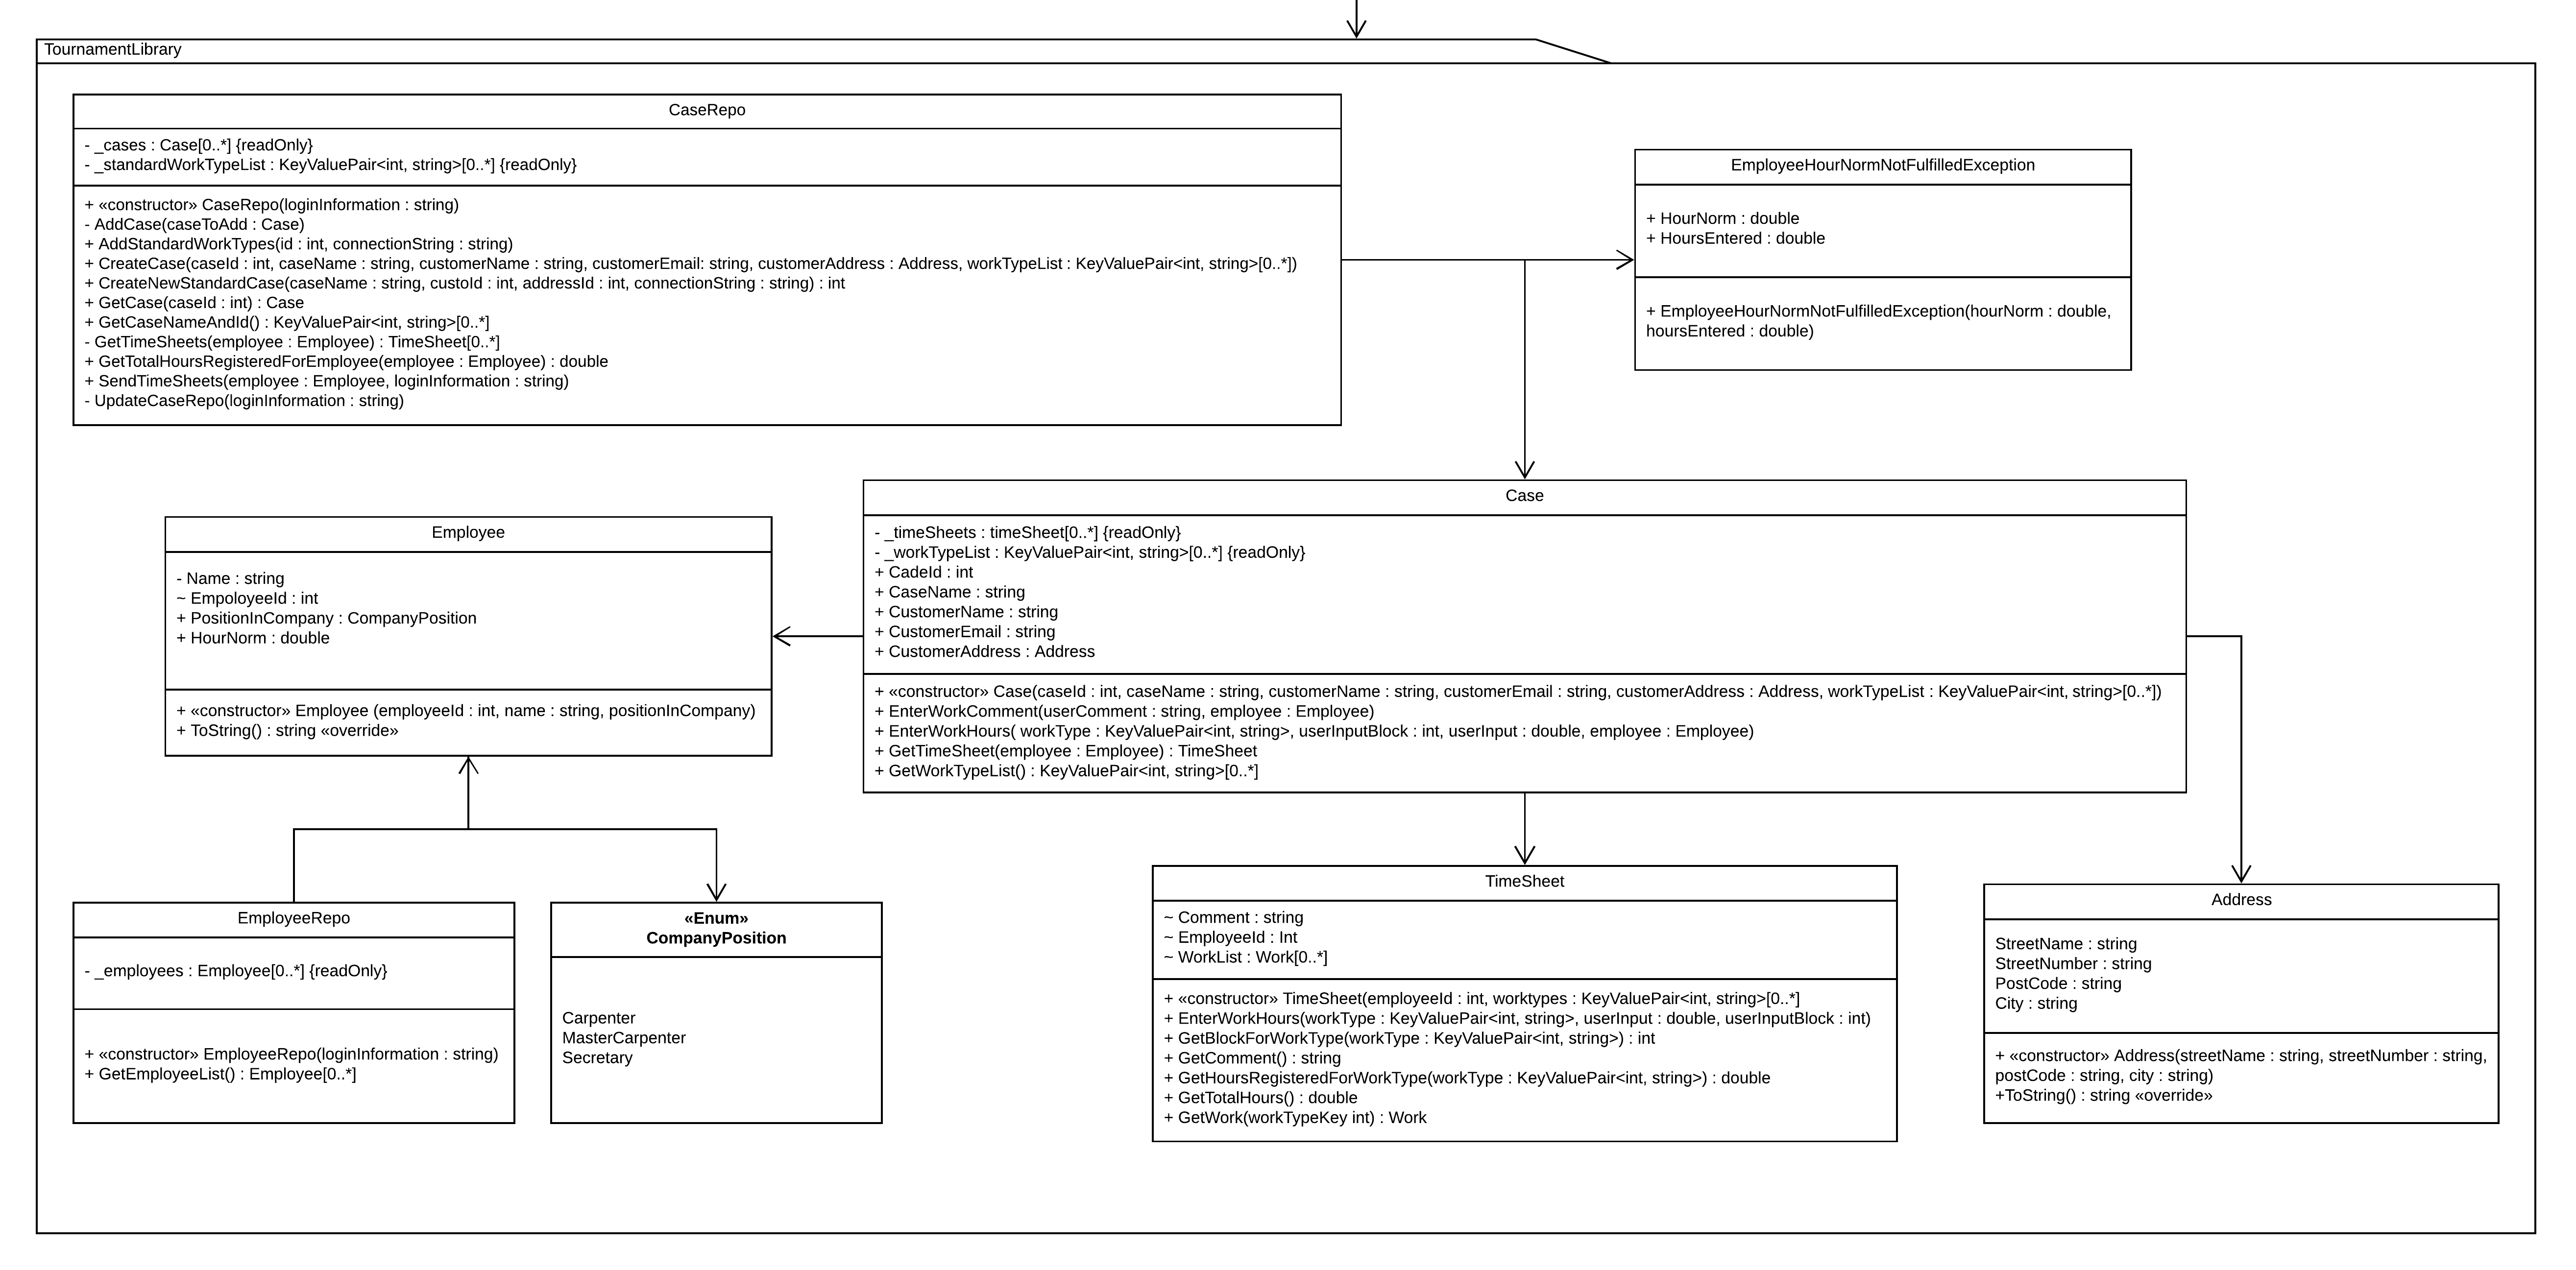
\includegraphics[scale = .6]{DCDTimeregistration.png}}
    \caption{DCD for TournamentLibrary Namespacet.}
    \label{fig:DCDLib}
\end{figure}